\chapter{Results: methods comparison}

\textbf{colocar resultados y plots de comparacion}

In this chapter we will study different data sets using the two presented methods for the \textit{BGSEES} algorithm: the \textbf{Least Squares} and \textbf{Decrease Range} method. 

The aim of the chapter is to test them against each other and using different parameters to see which method yields the best result

The algorithm is tested using data from both Solar flares and flares from far-away stars. Because the day hemisphere has to be discarded in order to study far-away stars (because of the Sun's effect on the ionosphere), the first section will study examples of flares originating from the Sun and the second those from outside the Solar System. -> En este capitulo al final solo sol, estrellas en el siguiente

For the solar flares, the ti files of days when a flare had taken place were used to compare the results. The data was filtered around the time of the flare (30 minutes before and after, if there was an exact moment in time).
 
Below is the list of times (\textit{year.day.seconds}) of the different flares we studied. The seconds are either an exact moment in time or a range used in the plots of the papers the flares are listed in.

Flares listed in \textit{"GNSS measurement of EUV photons flux rate during strong and mid solar flares"}\cite{hernandez2012gnss}

LA LISTA HA CAMBIADO

\begin{itemize}
	\item 2003.301.39777
	\item 2003.308.71000-71100
	\item 2005.020.24200-24400
	\item 2006.340.67300-67500
	\item 2011.210.44134
	\item 2011.216.13908
\end{itemize}

And those listed in \textit{"GPS as a solar observational instrument: Real-time estimation of EUV photons flux rate during strong, medium, and weak solar flares"}\cite{singh2015gps}

\begin{itemize}
	\item 2001.334.3700-4000
	\item 2001.347.51800-52200
	\item 2002.196.72240
	\item 2004.204.27800-28000
	\item 2004.310.41370
	\item 2004.313.52500
	\item 2005.258.30990
	\item 2012.066.4400-4700
	\item 2012.130.50600-51000
	\item 2012.297.11600-12000
	\item 2013.310.35970
\end{itemize}

To perform this study, the best epoch within the given range is found using the mean VTEC, as shown in chapter 5. The data is then filtered using this epoch and the algorithm is executed using the necessary parameters, the studied factors are:

The \textbf{execution time} of the algorithm and the \textbf{absolute error} of the estimation, obtained by computing the angle between correct Sun position\footnote{The correct Sun position at that moment is obtained from the data, it is one of the many fields the ti files contain} and the estimated location, using the same operations we've used in previous chapters to compute the angle. 

The ti files that contain data for the entire day are filtered using this bash script, which has a list with the information of each file to be filtered: the name of the original file and the upper and lower limits of time (or a specific moment used to compute the limits). It then filters each file using a simple AWK one-line script that checks the field with the time:

\begin{minipage}{\linewidth}
	\begin{lstlisting}[language=Bash, caption=Filtering the ti file]
#!/bin/bash	
	
strings=(
	'2003.301,36000,41400'
	'2011.210,44134'
	[..All the filenames..] 
	'2012.130,50600,51000'
	'2012.297,11600,12000'
)

tiDataFolder="/home/mbdavid2/Documents/dataTi/"

for i in "${strings[@]}"; do
	dataInfo="$i"
	
	# Split the information
	arrayInfo=(${dataInfo//,/ })
	
	# Use the range if specified, compute it otherwise
	if [ ${#arrayInfo[@]} = 2 ]; then
		let lowerLimit="${arrayInfo[1]}"-1800
		let upperLimit="${arrayInfo[1]}"+1800
	else
		let lowerLimit="${arrayInfo[1]}"
		let upperLimit="${arrayInfo[2]}"
	fi
	
	# Name the file according to the parameters
	tiDataFile="ti.""${arrayInfo[0]}"
	outputFileName="$tiDataFile"".""$lowerLimit""-""$upperLimit"
	echo $outputFileName
	
	# Filter and compress
	zcat "$tiDataFolder""originals/""$tiDataFile" 
	| gawk -v lower="$lowerLimit" -v upper="$upperLimit" 
	'{/a/; if ($3 >= lower/3600 && $3 <= upper/3600) {print $0;}}' 
	> "$tiDataFolder""$outputFileName"
	gzip -f "$tiDataFolder""$outputFileName" # -f to force overwrite
done\end{lstlisting}
\end{minipage}

The study is divided in three categories, based on the method used to discard outliers from the input data:

\begin{itemize}
	\item Using the data from \textbf{all IPPs} without filtering out any outliers
	\item Using a \textbf{cutoff value} for the VTEC only when \textbf{finding the spike}
	\item Using a \textbf{cutoff value} for \textbf{all the VTEC data} that will be used for the computations of the algorithm (si ???)
	\item Using \textbf{linear fit} for the Decreasing Range method to discard outliers and \textbf{multiple iterations} for the Least Squares method to try to improve the solution, both explained in their respective chapters.
\end{itemize}

\section{Using all available data}

For this first test, all the data from the ti file is used: in the case of the Decreasing Range (DR) method, all the VTEC values that could be invalid are used to compute the correlation, and in the case of the Least Squares (LS) method, all are used for the equations of the system.

\begin{table}[h!]
	\centering
	\def\arraystretch{1.2}
	\begin{tabular}{|c c c|} 
		\hline
		Data set & Total estimation error (degrees) & Time (seconds) \\ [0.5ex] 
		\hline\hline
		ti.2001.347.gz & 113.813 & 1.03879 \\
		\hline
		ti.2002.196.gz & 83.5147 & 0.26934 \\
		\hline
		ti.2003.301.gz & 24.6405 & 1.07813 \\
		\hline
		ti.2003.308.gz & 128.59 & 0.971644 \\
		\hline
		ti.2005.020.gz & 20.1031 & 0.916863 \\
		\hline
		ti.2005.258.gz & 91.3298 & 0.498707 \\
		\hline
		ti.2011.210.gz & 90.5716 & 1.46812 \\
		\hline
		ti.2012.066.gz & 133.236 & 2.30571 \\
		\hline
		ti.2012.130.gz & 162.888 & 2.49292 \\
		\hline
		ti.2012.297.gz & 78.487 & 0.789705 \\
		\hline\hline
		Total & 927.174 & 11.8299 \\
		\hline
	\end{tabular}
	\caption{Estimation error and execution time for different data sets using the DR method without any filter}
\end{table}

\begin{table}[h!]
	\centering
	\def\arraystretch{1.2}
	\begin{tabular}{|c c c|} 
		\hline
		Data set & Total estimation error (degrees) & Time (seconds) \\ [0.5ex] 
		\hline\hline
		ti.2001.347.gz & 106.064 & 0.0175844 \\
		\hline
		ti.2002.196.gz & 66.2043 & 0.0158694 \\
		\hline
		ti.2003.301.gz & 42.2689 & 0.0154119 \\
		\hline
		ti.2003.308.gz & 55.4949 & 0.326298 \\
		\hline
		ti.2005.020.gz & 124.218 & 0.14858 \\
		\hline
		ti.2005.258.gz & 111.073 & 0.0264138 \\
		\hline
		ti.2011.210.gz & 98.776 & 0.0558694 \\
		\hline
		ti.2012.066.gz & 64.186 & 0.0143492 \\
		\hline
		ti.2012.130.gz & 73.1871 & 0.0321778 \\
		\hline
		ti.2012.297.gz & 47.0189 & 0.00680915 \\
		\hline\hline
		Total & 788.491 & 0.659363 \\
		\hline
	\end{tabular}
	\caption{Estimation error and execution time for different data sets using the LS method without any filter}
\end{table}

\subsection{Discussion}

The main problem of this method is that outliers can cause the computation of the mean to be unstable, which causes the algorithm to use incorrect epochs. Furthermore, the outliers can cause numerical instability in some of the methods' computations, if one has a large value, for example, the computation of the correlation relies on the sum of the square of the VTEC value, so the total can lead to incorrect results.

Another thing that we can see, is that the LS method is significantly faster: all data sets together add up to a total execution time of less than one second, whilst the DR method needs that time or even more for almost each of the data sets.

\section{Direct VTEC filter}

Although this is a very simple method to discard outliers, it works because the value of the VTEC does not usually surpass values such as 0.8, although some IPPs present measures like this, perhaps due to other interferences in the satellite data. The flare from the day 301 of 2003, for example, studied in previous chapters, is one of the most powerful flares ever recorded, and the peak value of the Delta VTEC is 0.4.

These are the results of the execution using a cutoff value of 0.7. This value was selected as it is the one that yielded the best results in a range of 0.3 to 1.

\begin{table}[h!]
   	\centering
   	\def\arraystretch{1.2}
   	\begin{tabular}{|c c c|} 
   		\hline
   		Data set & Total estimation error (degrees) & Time (seconds) \\ [0.5ex] 
   		\hline\hline
   		ti.2001.347.gz & 3.53947 & 1.03243 \\
   		\hline
   		ti.2002.196.gz & 27.6877 & 0.287287 \\
   		\hline
   		ti.2003.301.gz & 3.93239 & 1.36538 \\
   		\hline
   		ti.2003.308.gz & 131.366 & 0.891328 \\
   		\hline
   		ti.2005.020.gz & 64.8737 & 0.551884 \\
   		\hline
   		ti.2005.258.gz & 48.7806 & 1.00214 \\
   		\hline
   		ti.2011.210.gz & 126.204 & 1.23266 \\
   		\hline
   		ti.2012.066.gz & 75.1081 & 1.85402 \\
   		\hline
   		ti.2012.130.gz & 56.7937 & 2.42187 \\
   		\hline
   		ti.2012.297.gz & 1.46042 & 2.86145 \\
   		\hline
   		\hline
   		Total & 539.746 & 13.5005 \\
   		\hline
   	\end{tabular}
   	\caption{Estimation error and execution time for different data sets using the DR method with a cutoff filter}
\end{table}

\subsection{Least Squares}

\begin{table}[h!]
   	\centering
   	\def\arraystretch{1.2}
   	\begin{tabular}{|c c c|} 
   		\hline
   		Data set & Total estimation error (degrees) & Time (seconds) \\ [0.5ex] 
   		\hline\hline
   		ti.2001.347.gz & 3.41832 & 0.0114944 \\
   		\hline
   		ti.2002.196.gz & 46.578 & 0.00492704 \\
   		\hline
   		ti.2003.301.gz & 4.57509 & 0.00724225 \\
   		\hline
   		ti.2003.308.gz & 141.865 & 0.378145 \\
   		\hline
   		ti.2005.020.gz & 38.3263 & 0.129509 \\
   		\hline
   		ti.2005.258.gz & 1.88011 & 0.0103007 \\
   		\hline
   		ti.2011.210.gz & 38.5213 & 0.0603164 \\
   		\hline
   		ti.2012.066.gz & 70.1063 & 0.0251154 \\
   		\hline
   		ti.2012.130.gz & 9.26238 & 0.0518934 \\
   		\hline
   		ti.2012.297.gz & 3.00704 & 0.0392889 \\
   		\hline\hline
   		Total & 357.54 & 0.718233 \\
   		\hline
   	\end{tabular}
   	\caption{Estimation error and execution time for different data sets using the LS method with a cutoff filter}
\end{table}

\subsection{Discussion}

As we can see

Considering how for both cases using the direct filter yields significantly better results, the next sections use this for filtering the first traversal of the data.

\section{Decreasing range: linear fit}

explain: best combination 3 y 4?

\begin{table}[h!]
	\centering
	\def\arraystretch{1.2}
	\begin{tabular}{|c c c|} 
		\hline
		Data set & Total estimation error (degrees) & Time (seconds) \\ [0.5ex] 
		\hline\hline
		ti.2001.347.gz & 3.66657 & 45.4151 \\
		\hline
		ti.2002.196.gz & 30.9237 & 42.6182 \\
		\hline
		ti.2003.301.gz & 3.57674 & 51.7222 \\
		\hline
		ti.2003.308.gz & 79.3679 & 43.6955 \\
		\hline
		ti.2005.020.gz & 68.911 & 37.3023 \\
		\hline
		ti.2005.258.gz & 22.6375 & 50.5795 \\
		\hline
		ti.2011.210.gz & 19.7344 & 55.8291 \\
		\hline
		ti.2012.066.gz & 84.3076 & 31.9302 \\
		\hline
		ti.2012.130.gz & 21.896 & 42.326 \\
		\hline
		ti.2012.297.gz & 0.679492 & 53.7369 \\
		\hline
		Total & 335.701 & 455.155 \\
		\hline
	\end{tabular}
	\caption{Results for different data sets}
\end{table}

\section{Least Squares: Iterations}

10 iterations, saves the result of the best iteration.

\begin{table}[h!]
	\centering
	\def\arraystretch{1.2}
	\begin{tabular}{|c c c|} 
		\hline
		Data set & Total estimation error (degrees) & Time (seconds) \\ [0.5ex] 
		\hline\hline
		ti.2001.347.gz & 3.41832 & 0.0194832 \\
		\hline
		ti.2002.196.gz & 46.578 & 0.00818968 \\
		\hline
		ti.2003.301.gz & 4.57509 & 0.0171783 \\
		\hline
		ti.2003.308.gz & 141.865 & 0.366494 \\
		\hline
		ti.2005.020.gz & 38.3263 & 0.141508 \\
		\hline
		ti.2005.258.gz & 1.88011 & 0.0177967 \\
		\hline
		ti.2011.210.gz & 38.5213 & 0.0704044 \\
		\hline
		ti.2012.066.gz & 70.1063 & 0.049831 \\
		\hline
		ti.2012.130.gz & 9.26238 & 0.0711422 \\
		\hline
		ti.2012.297.gz & 3.00704 & 0.0592826 \\
		\hline
		Total & 357.54 & 0.82131 \\
		\hline
	\end{tabular}
	\caption{Results for different data sets}
\end{table}

As we can see, the results in terms of estimation error are exactly the same as the ones seen in table \ref{tab:lsDirect} with a slight increase in execution time due to the number of iterations. Because there is no improvement with consecutive iterations, the algorithm just keeps the best result from the first one, hence the same results.

\section{Least Squares estimation error}

As we have seen in the previous chapter, using the estimation error to find the best estimation does not work because.... But it can be interesting to see how the estimation error evolves compared to the real error for all the studied data sets, the following plot shows:

\begin{figure}[!htb]
	\begin{centering}
		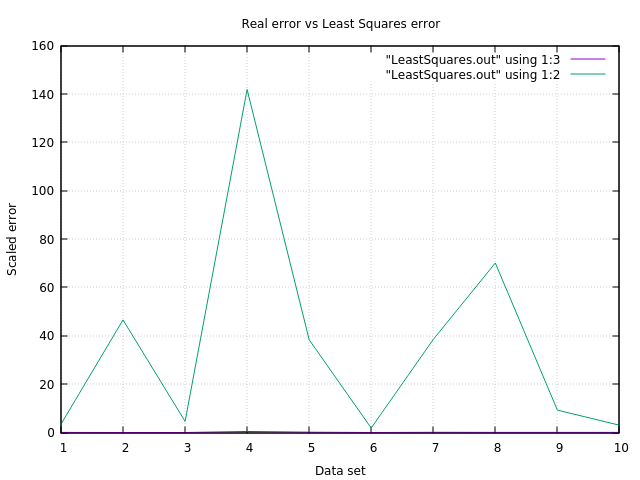
\includegraphics[width=0.5\linewidth]{images/results/comparisonErrors.png}
		\caption{Comparison of the real error and the estimated Least Squares error}
		\label{fig:comparisonErrors}
	\end{centering}
\end{figure}

\section{Conclusion}

conclusion de todo el chapter?

